\documentclass{article}
\usepackage{graphicx}
\usepackage[a4paper, margin=1in]{geometry}
\usepackage{hyperref}
\graphicspath{{assets/}}

\title{P2P Chat and VoIP Application using UDP in Java}

\author{
    \small Aristotle University of Thessaloniki - Department of Electrical and Computer Engineering \\[0.5em]
    \small Computer Networks II\\[1.5em]
    Epameinondas Bakoulas and Maria Sotiria Kostomanolaki \\[1em]
}

\date{December 2024}

\begin{document}

\maketitle

\begin{abstract}
This report presents the development of a Peer-to-Peer (P2P) Chat and Voice over IP (VoIP) application, created as part of the Computer Networks II course at Aristotle University of Thessaloniki. The application uses Java's \texttt{java.net} library for network communications, providing hands-on experience with real-time data exchange and concurrency. Designed for communication between two peers, it supports instant messaging and multimedia data transfer.

The project also explores the concept of switching between UDP and TCP protocols to understand their trade-offs. Although implementing the switch to TCP did not result in a functional feature, this exploration deepened our understanding of Internet Protocols, challenges posed by NAT (Network Address Translation), and the role of port forwarding in enabling P2P communication. Additionally, cryptographic techniques were integrated to secure the exchanged data, emphasizing the importance of privacy in P2P communication.
\end{abstract}

\section {UDP Chat and VoIP Application}

\subsection{Variables}
The application uses two \texttt{DatagramSocket} objects:
\begin{itemize}
    \item \texttt{messageSocket} for handling message communication
    \item \texttt{voiceSocket} for handling voice data
\end{itemize}
This separation is important to avoid conflicts between the different types of data (text and voice) that are transmitted over UDP, 
as each socket is dedicated to a specific purpose. Additionally, the application uses four \texttt{ports}:
\begin{itemize}
    \item \textbf{Local Ports}: \texttt{LOCAL\_PORT\_MESSAGE (12345)} is used for receiving messages, and \texttt{LOCAL\_PORT\_VOICE (12346)} is used 
    for receiving voice data. Each type of communication (messages and voice) requires a dedicated port to \textbf{listen} for incoming data.
    \item \textbf{Remote Ports}: \texttt{REMOTE\_PORT\_MESSAGE (12345)} is used for sending messages to the remote peer, and \texttt{REMOTE\_PORT\_VOICE (12346)} 
    is used for sending voice data. These ports ensure that data is \textbf{sent} to the appropriate destination, depending on whether it is a message or voice.
\end{itemize}
This setup enables efficient, organized handling of different data streams (text vs. voice) and ensures that there are no interference or 
data delivery issues for each type of communication.

\subsection{Initialization Process and Socket Management}
The application ensures efficient resource management and smooth communication by dynamically handling socket initialization. Below is an 
itemized explanation of the initialization process:

\begin{enumerate}
\item \textbf{Default UDP Initialization:}
        \begin{itemize}  
        \item Method Used: \texttt{initUDPSockets()}
        \item When Used: On app startup or when the user switches to UDP via the protocol switch button.
        \item What It Does: Creates and binds UDP sockets for messaging and voice communication using predefined local ports. This allows the app to start 
        communication immediately using the UDP protocol.
        \end{itemize}

\item \textbf{Releasing Resources:}
        \begin{itemize}
        \item Methods Used: \texttt{deinitUDPSockets()} and \texttt{deinitTCPSockets()} 
        \item When Used: Before switching to a different protocol.
        \item What It Does: Ensures that sockets from the inactive protocol are properly closed, freeing up the associated resources and avoiding conflicts on the same ports.
        \end{itemize}
\end{enumerate}
This modular approach minimizes resource usage, prevents port conflicts, and allows seamless protocol switching without restarting the application.\

\section{Encryption}
The application uses the \texttt{AES} (Advanced Encryption Standard) algorithm to secure data exchanged between peers. The encryption key is hardcoded within the application and is used for both encrypting and decrypting messages. For optimal security, the key should be exchanged between peers securely to maintain the privacy and integrity of the communication.

While the implementation does not currently include a secure key exchange mechanism, methods such as the \texttt{Diffie-Hellman} key exchange protocol can be employed to securely share encryption keys between peers in a real-world scenario. This is an important consideration for ensuring private communication over potentially insecure networks.

Additionally, an example of the encrypted payload produced by the application can be seen in Section 4, Figures 3 and 4, which illustrate how data is transformed through encryption. This highlights the practical application of the encryption process within the system.

\section{Fullstack Application}
Using the Java framework \texttt{Spring Boot} for the backend and the frontend library \texttt{React}, we developed a full-stack application. Each backend instance is designed to communicate exclusively with a single frontend instance, ensuring secure and end-to-end communication.

The backend exposes its functionality through REST APIs, which the frontend consumes using the \texttt{Axios} library. This architecture facilitates efficient and structured interaction between the client and server, enabling seamless real-time data exchange.

To run the application, both the backend and frontend servers need to be started:
\begin{itemize}
    \item \textbf{Backend Server}: Run the command \texttt{mvn spring-boot:run}.
    \item \textbf{Frontend Server}: Run the command \texttt{npm run dev}.
\end{itemize}

For users who prefer not to launch the full-stack application, an alternative standalone GUI application can be run by executing the \texttt{App.java} file. This approach bypasses the need for server setups.

The core files of the full-stack application are:
\begin{itemize}
    \item \texttt{AppController.java}: Handles backend logic and API endpoints.
    \item \texttt{App.jsx}: Implements the main frontend component.
\end{itemize}

The chat application user interface can be seen in Figure 1.

\begin{figure}[h!]
    \centering
    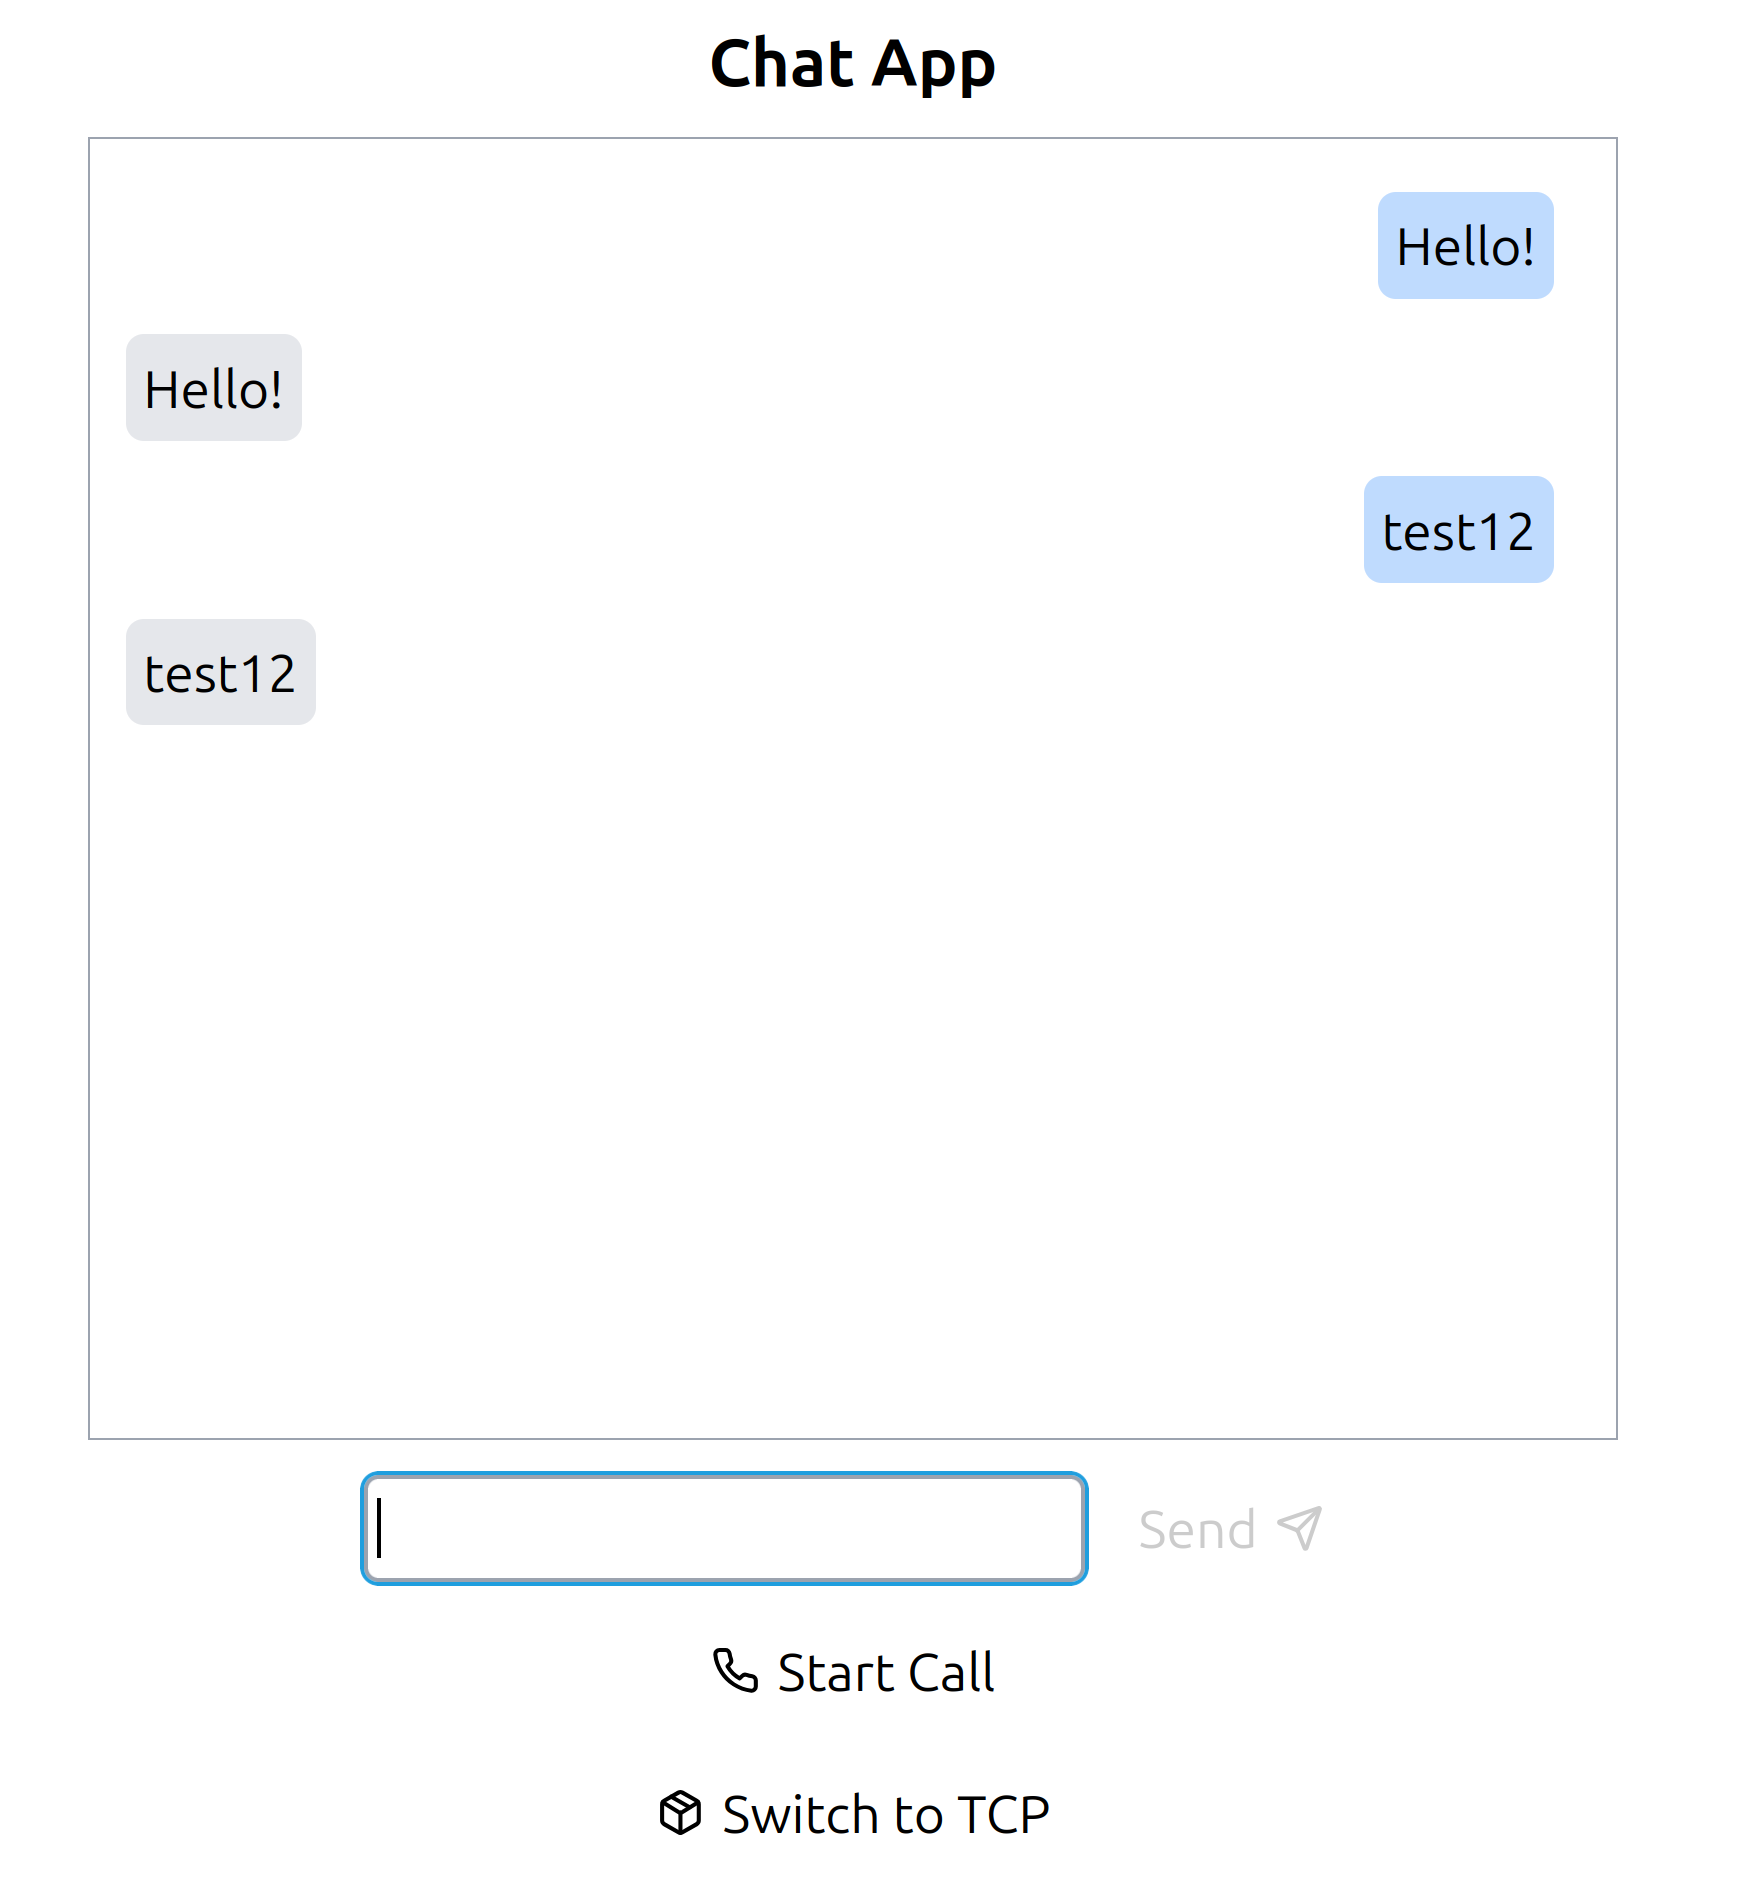
\includegraphics[width=0.5\textwidth]{chat1.png}
    \caption{Chat Application User Interface}
    \label{fig:chat1}
\end{figure}

\section{Wireshark packets}

\subsection{Port Forwarding}

To test the functionality of our application in a remote setting, we utilized \textbf{port forwarding} by creating a custom rule in the NAT and Security settings of our personal Wi-Fi routers. This configuration allowed us to redirect incoming traffic to the appropriate device within our local networks.

In addition to setting up port forwarding, testing required temporarily disabling the firewall on both devices to ensure that the network traffic was not blocked. After exchanging our public IP addresses, we configured the code accordingly by:
\begin{itemize}
    \item Setting the \texttt{REMOTE\_IP} variable to the IP address of the other peer.
    \item Adjusting the number of ports used for communication to match the settings configured in the port forwarding rules.
\end{itemize}

With these configurations in place, we successfully tested the application's functionality remotely, exchanging messages between two devices across different networks.

\subsection{UDP Messages Packets}

After successfully establishing communication between our two devices and exchanging several messages, we used \textbf{Wireshark} to analyze the network traffic and demonstrate the functionality of the application. The messages exchanged are encrypted using the \texttt{AES} algorithm, ensuring the privacy of the communication. The encryption key used for this process is \texttt{123456789ABCDEFG}.

In Figure 2, we observe the packets being sent and received between the two devices, identified by their distinct IP addresses. This confirms the proper transmission of data between peers. Figures 3 and 4 further illustrate the encryption in action by showing the encrypted payload of the messages. These encrypted messages highlight the security measures implemented in the application, ensuring that sensitive data remains private and inaccessible to unauthorized parties.

\begin{figure}[h!]
    \centering
    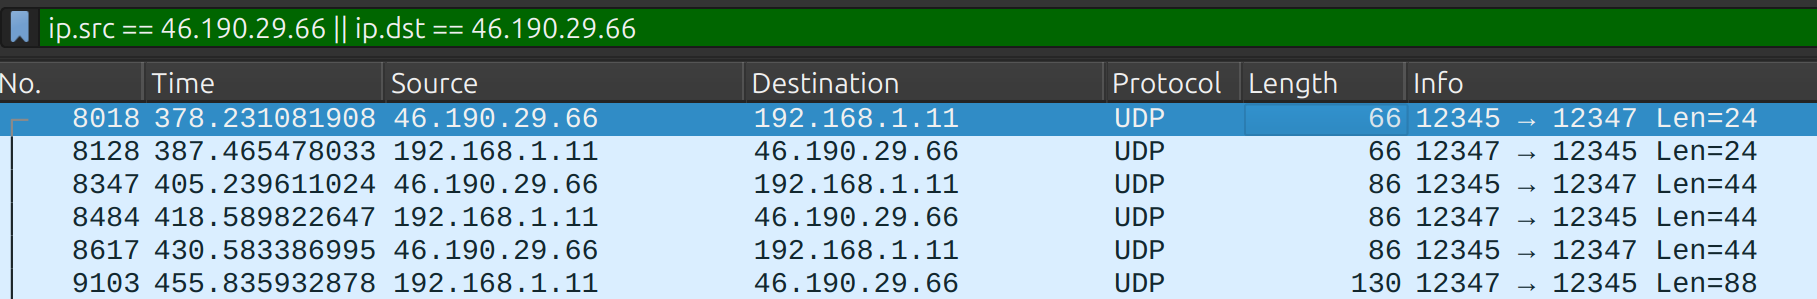
\includegraphics[width=0.8\textwidth]{udp-messages-1.png}
    \caption{UDP message packet exchanging with port forwarding}
    \label{fig:udp-messages-1}
\end{figure}

\begin{figure}[h!]
    \centering
    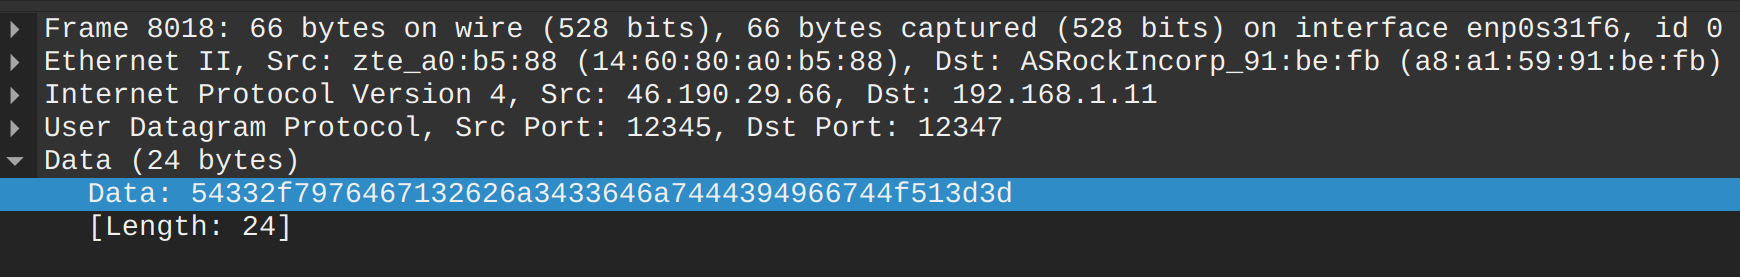
\includegraphics[width=0.8\textwidth]{udp-messages-2.png}
    \caption{UDP message packet (encrypted Payload marked)}
    \label{fig:udp-messages-2}
\end{figure}

\begin{figure}[h!]
    \centering
    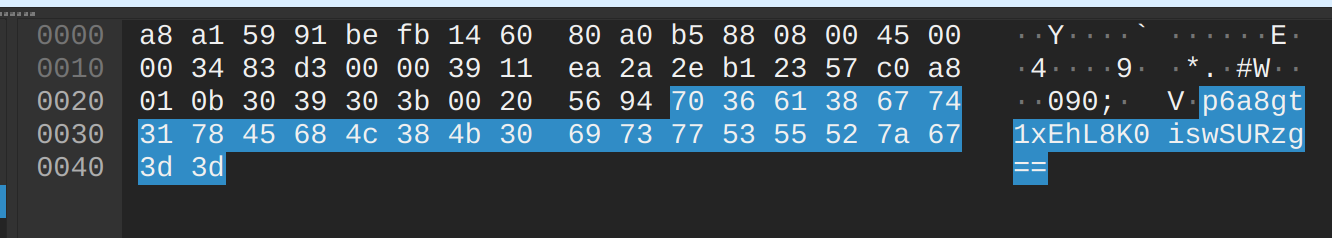
\includegraphics[width=0.8\textwidth]{udp-messages-3.png}
    \caption{UDP message packet (encrypted Payload marked)}
    \label{fig:udp-messages-3}
\end{figure}

\newpage We can also observe that messages larger than the Maximum Transmission Unit (MTU) size of UDP packets are fragmented and reassembled on the receiver, as shown in Figure 5. This process of fragmentation and reassembly is inherent to UDP communication when transmitting data that exceeds the MTU size.


\begin{figure}[h!]
    \centering
    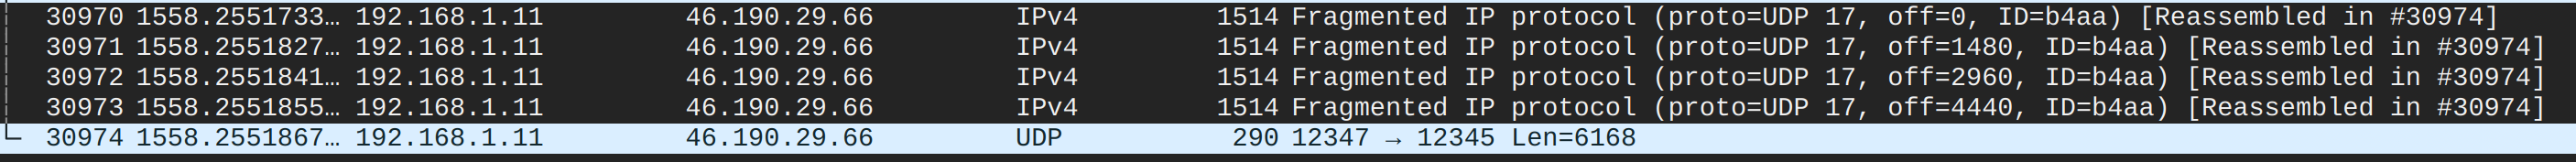
\includegraphics[width=0.8\textwidth]{udp-messages-fragmented.png}
    \caption{Large UDP message fragmented}
    \label{fig:udp-messages-4}
\end{figure}

\subsection{UDP Voice Packets}

The application supports the exchange of voice data, enabling a form of voice calling between peers. Once both peers activate this feature by pressing the call button, the application establishes a continuous exchange of voice packets (as shown in Figure 6).

\begin{figure}[h!]
    \centering
    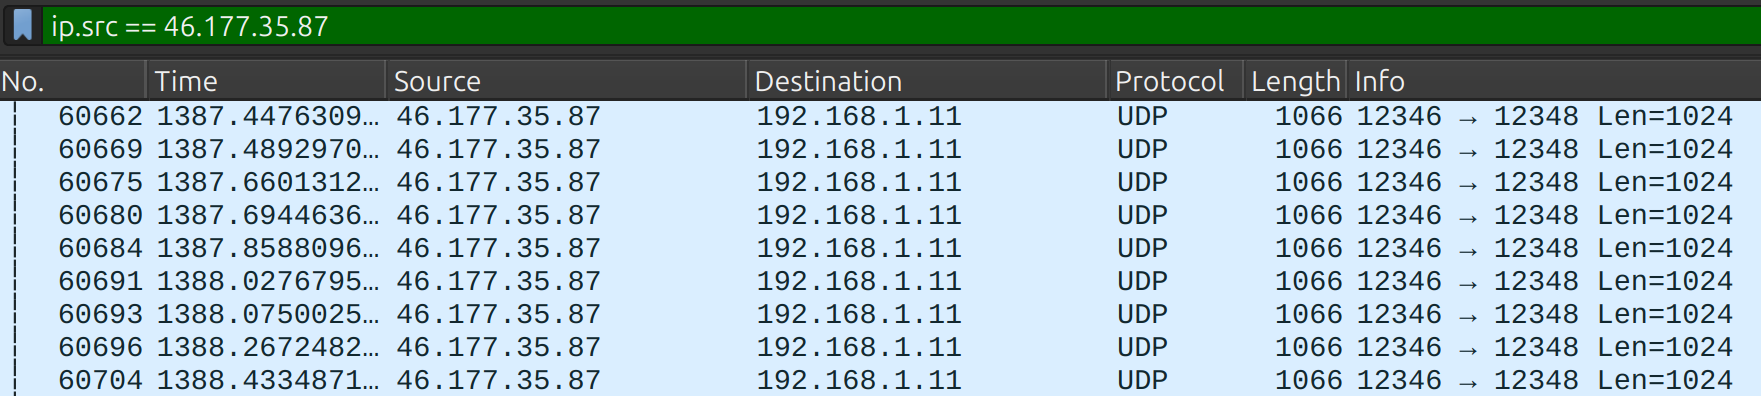
\includegraphics[width=0.8\textwidth]{udp-voice-1.png}
    \caption{UDP continuous voice packets}
    \label{fig:udp-voice-1}
\end{figure}

The voice packets are sent in a continuous stream and stored on the receiving end using a 1024-byte buffer. This buffer temporarily holds the incoming voice data, which is then played back to the user through the \texttt{SourceDataLine} class. The continuous exchange of voice packets stops when the user presses the call button again to end the call. Figures 7 and 8 provide a detailed view of the payload of these voice packets, showcasing the structure and data content exchanged during the voice call.

\begin{figure}[h!]
    \centering
    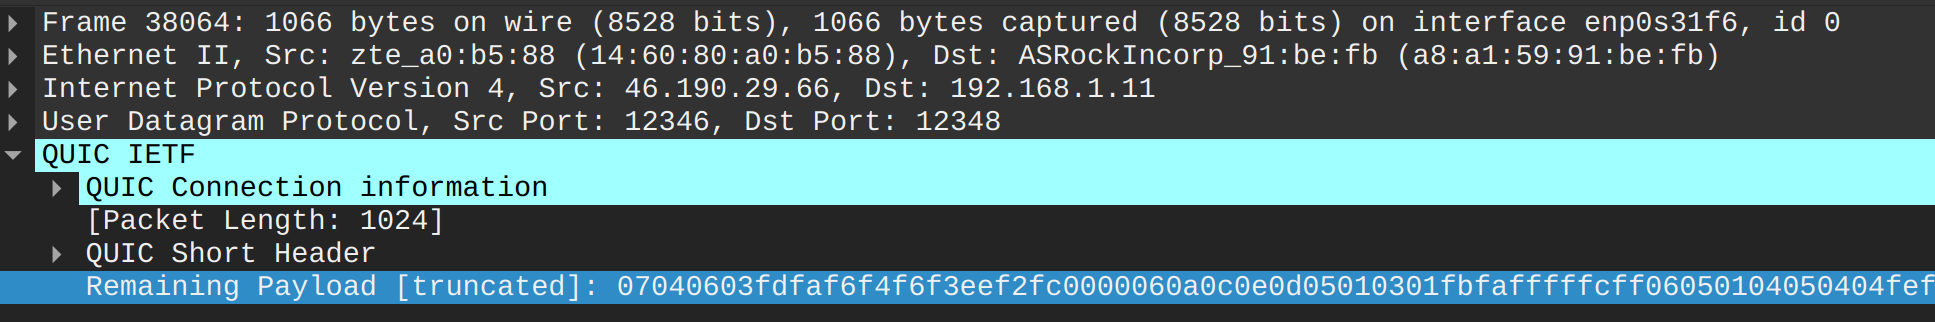
\includegraphics[width=0.8\textwidth]{udp-voice-2.png}
    \caption{UDP voice packet (Payload marked)}
    \label{fig:udp-voice-2}
\end{figure}

\begin{figure}[h!]
    \centering
    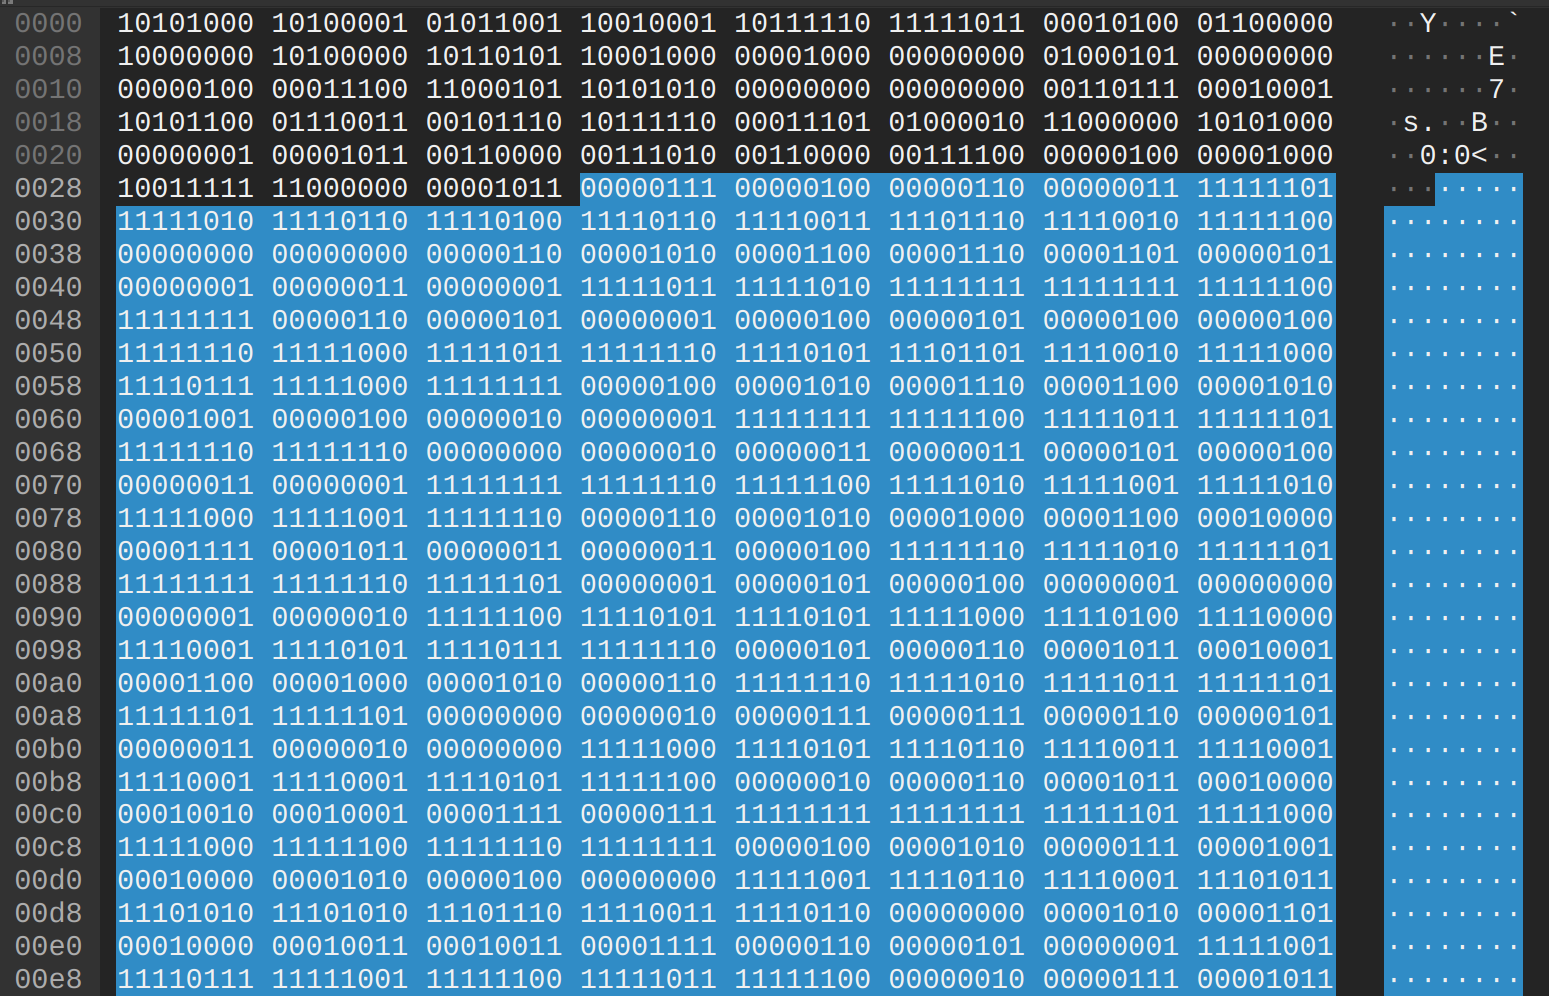
\includegraphics[width=0.8\textwidth]{udp-voice-3.png}
    \caption{UDP voice packet (Payload marked)}
    \label{fig:udp-voice-3}
\end{figure}

\section{TCP Implementation and Protocol Switching}

In this project, we explored the implementation of a TCP connection as an alternative to the existing UDP-based communication. To achieve this, we used the following sockets on both sides of the communication:

\begin{itemize}
    \item \texttt{tcpMessageServerSocket}: Server-side TCP socket for messaging.
    \item \texttt{tcpMessageSocket}: Client-side TCP socket for messaging.
    \item \texttt{tcpVoiceServerSocket}: Server-side TCP socket for voice.
    \item \texttt{tcpVoiceSocket}: Client-side TCP socket for voice.
\end{itemize}

To integrate protocol switching into the application, we added a protocol switch button to the user interface. This button was designed to allow users to toggle between UDP and TCP protocols for both messaging and voice functionalities. However, despite our efforts, we were unable to overcome the challenges posed by P2P communication and successfully establish a TCP connection. These challenges were primarily related to the barriers introduced by Network Address Translation (NAT) and other network constraints.

Although the TCP implementation did not result in a functional connection, this exploration deepened our understanding of IP protocols and the complexities involved in establishing P2P communication using TCP. The reader is encouraged to review the code to gain further insights into the attempted implementation and the obstacles encountered.


\section{References}
\begin{itemize}
    \item GitHub Repository: \url{https://github.com/NontasBak/CN2_AUTH_ChatAndVoIP}
\end{itemize}

\end{document}